\documentclass[a4paper,12pt]{report}

% Codifica e lingua
\usepackage[utf8]{inputenc}
\usepackage[T1]{fontenc}
\usepackage[italian]{babel}
\usepackage{float}

% Formattazione
\usepackage{geometry}
\geometry{margin=2.5cm}
\usepackage{graphicx}
\graphicspath{{img/}}
\usepackage{hyperref}
\usepackage[all]{hypcap}
\usepackage{url}
\usepackage{listings}
\usepackage{xcolor}

% Kotlin syntax highlighting
\definecolor{kotlinpurple}{rgb}{0.4,0.0,0.6}
\definecolor{kotlinblue}{rgb}{0.0,0.3,0.7}
\definecolor{kotlingreen}{rgb}{0.1,0.5,0.2}
\definecolor{kotlingray}{rgb}{0.5,0.5,0.5}

\lstdefinelanguage{Kotlin}{
  keywords={fun, val, var, class, object, interface, data, sealed, enum, when, if, else,
            return, override, private, public, internal, suspend, flow, collect, emit,
            launch, async, coroutineScope, viewModelScope, companion, by, lazy, init,
            null, true, false, is, as, in, out, abstract, open, final},
  keywordstyle=\color{kotlinpurple}\bfseries,
  stringstyle=\color{kotlinblue},
  commentstyle=\color{kotlingreen}\itshape,
  morecomment=[l]{//},
  morecomment=[s]{/*}{*/},
  morestring=[b]",
  basicstyle=\ttfamily\footnotesize,
  tabsize=4,
  showspaces=false,
  showstringspaces=false,
  frame=single,
  breaklines=true,
  postbreak=\mbox{\textcolor{red}{$\hookrightarrow$}\space},
}
\lstset{language=Kotlin}

% Link
\hypersetup{
    colorlinks=true,
    linkcolor=black,
    urlcolor=blue,
    pdftitle={Relazione di Progetto - StudentHub},
}

% Dati documento
\title{\textbf{Relazione di Progetto \\ ``StudentHub''}}
\author{Diego Andruccioli \and Giovanni Morelli \and Rei Mici}
\date{Anno Accademico 2025/2026}

% ============================================================
\begin{document}

\maketitle

% ── SOMMARIO ────────────────────────────────────────────────
\chapter*{Sommario}

StudentHub è un'applicazione Android per la gestione della carriera universitaria.
Lo studente registra i propri esami (nome, voto, CFU, data), consulta statistiche
sulla propria carriera accademica (media ponderata, media aritmetica, CFU totali,
proiezione della base di laurea) e monitora i propri progressi attraverso un sistema
di gamification: ogni esame superato genera punti esperienza (XP) calcolati dal server,
contribuisce all'avanzamento di livello e può sbloccare badge tematici.

L'applicazione è sviluppata interamente in Kotlin adottando Clean Architecture
multi-modulo, pattern MVVM con ViewModel e StateFlow, persistenza locale con
Room e DataStore, comunicazione REST tramite Retrofit e OkHttp, background
processing con WorkManager e interfaccia utente dichiarativa realizzata con Jetpack Compose.

La relazione è strutturata come segue: il Capitolo~1 presenta obiettivi e requisiti;
il Capitolo~2 illustra le scelte progettuali e le librerie adottate; il Capitolo~3
descrive i dettagli implementativi più significativi con il formato
Problema--Soluzione; il Capitolo~4 valuta punti forti e punti deboli del progetto;
il Capitolo~5 propone migliorie e sviluppi futuri.

\tableofcontents

% ── CAPITOLO 1 — OBIETTIVI E REQUISITI ──────────────────────
\chapter{Obiettivi e Requisiti}

\section{Descrizione del Progetto}

StudentHub nasce dall'esigenza di offrire allo studente universitario uno strumento
unico per la gestione della propria carriera accademica. Il dominio applicativo
comprende due aree distinte ma interconnesse: la gestione del libretto esami
(registrazione di voto, CFU e data per ciascun esame sostenuto, con calcolo automatico
di media ponderata, media aritmetica, CFU totali accumulati e proiezione della base
di laurea su 110) e la componente di gamification (assegnazione di punti XP a ogni
esame superato secondo la formula \textit{xp = voto × cfu + (lode ? 50 : 0)}
calcolata lato server, avanzamento di livello, sblocco di badge per traguardi raggiunti
e classifica degli studenti).

La logica di calcolo XP risiede esclusivamente nel backend Node.js, eliminando
duplicazioni e garantendo che i dati mostrati sull'app siano sempre allineati
con quelli ufficiali. L'applicazione è progettata per funzionare in modalità
offline-first: le operazioni sul libretto sono disponibili anche senza connessione
di rete e vengono sincronizzate con il server quando la connettività è ripristinata.

\section{Requisiti Funzionali}
\begin{itemize}
    \item Registrarsi con nome, cognome, e-mail e password per creare un nuovo account.
    \item Accedere con e-mail e password; la sessione viene ricordata tra un'apertura e l'altra dell'app.
    \item Visualizzare il libretto con la lista di tutti gli esami registrati, ordinati per data.
    \item Aggiungere un esame specificando nome, voto (18--30 con possibilità di lode), CFU e data.
    \item Eliminare un esame dal libretto.
    \item Visualizzare le statistiche della propria carriera (media ponderata, CFU totali, base di laurea, grafico andamento voti).
    \item Monitorare il completamento degli obiettivi di gamification e i punti XP guadagnati.
    \item Personalizzare le impostazioni dell'account (tema di colorazione dei voti, soglie RGB) nella schermata Profilo.
    \item Effettuare il logout dalla schermata Profilo; la sessione viene invalidata sia localmente che sul server.
    \item Ricevere una notifica locale quando il proprio rank nella classifica migliora.
\end{itemize}

\section{Requisiti Minimi del Corso}

I requisiti minimi obbligatori del corso Sistemi Mobili sono soddisfatti dall'applicazione
nei seguenti punti:

\begin{itemize}
    \item \textbf{Kotlin puro}: l'intero progetto è scritto in Kotlin; non è presente alcun file Java.
    \item \textbf{Separazione in moduli}: il codice è organizzato nei moduli \texttt{:domain},
          \texttt{:data}, \texttt{:ui} e \texttt{:app}, ciascuno con responsabilità distinte.
    \item \textbf{ViewModel e StateFlow}: ogni schermata utilizza un ViewModel dedicato
          come unico state holder; la UI osserva uno \texttt{StateFlow} tramite
          \texttt{collectAsStateWithLifecycle()} e non contiene logica di business.
    \item \textbf{Kotlin Coroutines}: tutte le operazioni di I/O (Room, chiamate di rete) avvengono
          su \texttt{Dispatchers.IO}; il Main Thread non viene mai bloccato.
    \item \textbf{Jetpack Compose}: l'interfaccia utente è implementata interamente in Jetpack
          Compose. Le liste di dati usano \texttt{LazyColumn} con chiave stabile per item,
          equivalente Compose di RecyclerView con DiffUtil.
    \item \textbf{Storage locale}: Room per la persistenza strutturata del libretto esami e dei
          dati di gamification; DataStore per le preferenze utente e i flag di onboarding.
    \item \textbf{Networking}: comunicazione REST con backend Node.js tramite Retrofit e OkHttp;
          autenticazione via cookie JWT HTTP-only con refresh automatico.
    \item \textbf{Background services}: WorkManager per la sincronizzazione offline degli esami
          e il controllo periodico del rank in classifica.
    \item \textbf{Runtime permission}: richiesta di \texttt{POST\_NOTIFICATIONS} (Android~13+)
          con dialog di rationale contestuale prima dell'invio della notifica.
    \item \textbf{Relazione finale}: questo documento.
\end{itemize}

% ── CAPITOLO 2 — SCELTE PROGETTUALI ─────────────────────────
\chapter{Scelte Progettuali}

\section{Architettura del Sistema}

\subsection{Clean Architecture Multi-Modulo}

Il progetto è strutturato in quattro moduli Gradle distinti, ciascuno con
responsabilità ben definite e dipendenze unidirezionali verso i layer inferiori.

\textbf{Modulo \texttt{:domain}} --- nucleo dell'applicazione. Contiene i modelli
di dominio (\texttt{Esame}, \texttt{User}, \texttt{Settings}, \texttt{GamificationStatus}),
le interfacce dei repository (\texttt{EsameRepository}, \texttt{AuthRepository},
\texttt{GamificationRepository}, \texttt{SettingsRepository}) e i Use Cases, ciascuno
con una sola responsabilità (\texttt{AddEsameUseCase}, \texttt{LoginUseCase},
\texttt{GetStatisticheUseCase}, ecc.). Il modulo è \emph{puro Kotlin}: non importa
nessuna classe Android, il che lo rende compilabile ed eseguibile in isolamento
su qualunque JVM. Questo è il principale vantaggio pratico: i test unitari dei
Use Cases e dei calcoli di business logic non richiedono un emulatore Android.

\textbf{Modulo \texttt{:data}} --- implementa le astrazioni definite in \texttt{:domain}.
Contiene le \texttt{@Entity} Room e i rispettivi \texttt{@Dao}, le implementazioni
dei repository (\texttt{EsameRepositoryImpl}, \texttt{AuthRepositoryImpl}, ecc.),
i client di rete (Retrofit API service, OkHttp con \texttt{PersistentCookieJar} e
\texttt{TokenAuthenticator}), i \texttt{DataStore} per preferenze e sessione, e i
\texttt{CoroutineWorker} di WorkManager. Nessuna Entity Room viene mai esposta al
di fuori di questo modulo: i mapper traducono Entity↔DomainModel al confine del layer.

\textbf{Modulo \texttt{:ui}} --- layer di presentazione realizzato interamente in
Jetpack Compose. Contiene i composable di schermata (\texttt{LibrettoScreen},
\texttt{StatisticheScreen}, \texttt{ObiettiviScreen}, \texttt{ProfiloScreen},
\texttt{LoginScreen}, \texttt{RegisterScreen}), i ViewModel e le sealed class
di stato UI (\texttt{LibrettoUiState}, \texttt{ProfiloUiState}, ecc.).
I ViewModel dipendono solo dalle interfacce del modulo \texttt{:domain}: non
importano mai classi Room o Retrofit direttamente.

\textbf{Modulo \texttt{:app}} --- punto di ingresso. Contiene \texttt{CustomApplication}
che implementa l'interfaccia \texttt{RepositoryProvider} e istanzia manualmente
tutti i repository, passando il \texttt{Context} necessario a Room e DataStore.
È l'unico modulo che dipende contemporaneamente da tutti gli altri.

\subsection{Schema delle Dipendenze tra Moduli}

\begin{verbatim}
:app  -->  :ui, :domain, :data
:ui   -->  :domain
:data -->  :domain
:domain --> (nessuna dipendenza interna)
\end{verbatim}

La freccia \texttt{:ui $\to$ :domain} e l'assenza di \texttt{:ui $\to$ :data}
sono la scelta progettuale più rilevante: il layer UI non può mai accedere
direttamente al database o al client di rete. Qualunque operazione sui dati
deve passare obbligatoriamente per un Use Case. Questa regola è applicata
strutturalmente dal sistema di build di Gradle: un tentativo di importare
una classe Room da un composable produrrebbe un errore di compilazione.

La freccia \texttt{:data $\to$ :domain} significa che le implementazioni
dei repository dipendono dalle interfacce definite nel dominio, non viceversa
(Dependency Inversion Principle): sostituire Room con un'altra soluzione di
persistenza richiederebbe modifiche solo in \texttt{:data}, lasciando intatti
\texttt{:domain} e \texttt{:ui}.

\subsection{Pattern MVVM e Flusso dei Dati}

Il flusso di un'azione utente procede in senso discendente attraverso i layer:

\begin{verbatim}
Composable --(evento)--> ViewModel --> UseCase --> Repository (interfaccia)
                                                        |
                                               RepositoryImpl --> Room DAO
                                                                   / Retrofit
\end{verbatim}

Il flusso reattivo dei dati procede in senso ascendente:

\begin{verbatim}
Room DAO: Flow<List<EsameEntity>>
    --> RepositoryImpl: map + flowOn(Dispatchers.IO)
    --> UseCase: trasformazioni business
    --> ViewModel: stateIn(viewModelScope, Eagerly) --> StateFlow<UiState>
    --> Composable: collectAsStateWithLifecycle()
\end{verbatim}

La UI non interroga mai attivamente i dati: osserva uno \texttt{StateFlow}
e si ridisegna per recomposition ogni volta che lo stato cambia.
Il ViewModel sopravvive ai cambi di configurazione (rotazione schermo,
ridimensionamento finestra) grazie al meccanismo di Jetpack: la connessione
al database Room non viene interrotta e lo stato dell'interfaccia viene
preservato senza richiedere logica aggiuntiva.

\section{Librerie e Tecnologie Utilizzate}

\subsection{Linguaggio e Ambiente di Sviluppo}

\begin{itemize}
    \item \textbf{Kotlin 2.2.10}: linguaggio ufficiale Android. Offre null safety,
    coroutine native, funzioni di estensione e data class rispetto a Java.
    \item \textbf{Android Studio}: IDE ufficiale con integrazione Gradle, debug su
    emulatore e profiler di memoria e CPU.
    \item \textbf{minSdk 31, targetSdk 36, Java 11 compatibility}: scelta che copre
    la grande maggioranza dei dispositivi Android attivi garantendo accesso alle API
    moderne (WorkManager, DataStore, Compose).
\end{itemize}

\subsection{Gestione delle Dipendenze}

\begin{itemize}
    \item \textbf{Gradle Kotlin DSL}: build script type-safe rispetto a Groovy;
    gli errori di configurazione vengono rilevati a compile-time.
    \item \textbf{Version Catalog (\texttt{libs.versions.toml})}: gestione
    centralizzata delle versioni. Una singola modifica al catalog aggiorna tutte
    le dipendenze omogenee nell'intero progetto multi-modulo.
    \item \textbf{KSP 2.3.2 (Kotlin Symbol Processing)}: processore di annotazioni
    per Room. Scelto rispetto a KAPT per la velocità di compilazione incrementale
    significativamente superiore con Kotlin 2.x.
\end{itemize}

\subsection{Jetpack e Librerie Core}

\begin{itemize}
    \item \textbf{Jetpack Compose (BOM 2025.12.00)}: toolkit UI dichiarativo.
    Elimina il file XML di layout, il ViewBinding e l'Adapter esplicito per le liste.
    Il composable \texttt{NavigationSuiteScaffold} gestisce la navigazione adattiva
    (Bottom Bar su smartphone, Navigation Rail su tablet) senza codice condizionale.

    \item \textbf{Room 2.7.2}: ORM per SQLite. Scelto rispetto all'accesso diretto
    a SQLite per le query type-safe, l'integrazione nativa con \texttt{Flow} e la
    gestione strutturata delle migration. Usato per il libretto esami e la cache
    locale dei dati di gamification.

    \item \textbf{DataStore Preferences 1.1.1}: persistenza chiave-valore asincrona.
    Scelto rispetto a \texttt{SharedPreferences} perché le operazioni sono sospensive
    (nessun rischio ANR) e l'API è basata su \texttt{Flow}. Usato per il flag di
    sessione (\texttt{is\_logged\_in}), le preferenze utente (tema voti, soglie RGB)
    e il rank in cache per le notifiche.

    \item \textbf{ViewModel + StateFlow (Lifecycle 2.8.7)}: state holder MVVM.
    Il ViewModel sopravvive alla rotation; lo \texttt{StateFlow} espone
    uno snapshot immutabile dello stato corrente alla UI.

    \item \textbf{Kotlin Coroutines + Flow 1.9.0}: modello di concorrenza strutturato.
    Obbligatorio per il corso: ogni operazione I/O avviene su \texttt{Dispatchers.IO},
    il Main Thread non viene mai bloccato.
\end{itemize}

\subsection{Librerie Aggiuntive}

\begin{itemize}
    \item \textbf{Retrofit 2.11.0 + OkHttp 4.12.0}: client HTTP per la comunicazione
    REST con il backend Node.js. OkHttp gestisce il ciclo di vita dei cookie JWT
    tramite \texttt{PersistentCookieJar} e il rinnovo automatico del token tramite
    \texttt{TokenAuthenticator}. Scelti rispetto ad \texttt{HttpURLConnection} per
    la leggibilità delle API Retrofit (interfacce Kotlin annotate) e per la ricchezza
    dell'ecosistema OkHttp (interceptor, authenticator, logging).

    \item \textbf{WorkManager 2.9.1}: scheduling garantito di task in background.
    Scelto rispetto ad \texttt{AlarmManager} perché gestisce automaticamente
    vincoli (connettività di rete), sopravvive ai riavvii del dispositivo e
    fornisce un'API Kotlin moderna con \texttt{CoroutineWorker}. Copre i requisiti
    d'esame per i background services.

    \item \textbf{Gson 2.11.0}: serializzazione JSON per la persistenza dei cookie
    OkHttp su \texttt{SharedPreferences}. Già presente come dipendenza transitiva
    di Retrofit; non aggiunge overhead al progetto.
\end{itemize}

% ── CAPITOLO 3 — DETTAGLI IMPLEMENTATIVI ─────────────────────
\chapter{Dettagli Implementativi}

\section{Gestione reattiva della lista esami}

\paragraph{Problema}
La lista degli esami deve aggiornarsi automaticamente ogni volta che un esame viene
aggiunto o eliminato, senza che la UI debba interrogare manualmente il database.
Un'implementazione basata su query one-shot richiederebbe un refresh esplicito
ad ogni operazione, con rischio di inconsistenze. È inoltre necessario evitare
memory leak quando il Fragment viene distrutto in seguito a un cambio di configurazione.

\paragraph{Soluzione}
Il pattern adottato sfrutta la reattività nativa di Room tramite \texttt{Flow}.
Il DAO espone \texttt{fun getAllEsami(): Flow<List<EsameEntity>>}: Room emette
automaticamente una nuova lista ad ogni modifica della tabella \texttt{esami}.
Il \texttt{RepositoryImpl} applica il mapper \texttt{toDomain()} e garantisce
l'esecuzione su \texttt{Dispatchers.IO} tramite \texttt{flowOn}.
Il \texttt{LibrettoViewModel} combina il Flow di Room con due \texttt{StateFlow}
di ordinamento (\texttt{\_sortBy}, \texttt{\_sortOrder}) tramite l'operatore
\texttt{combine()}, esponendo un unico \texttt{StateFlow<List<Esame>>} già ordinato.
Ogni variazione in uno qualunque dei tre flussi sorgente innesca automaticamente
un ricalcolo e una recomposition nella UI:

\begin{lstlisting}
private val _sortBy    = MutableStateFlow(SortBy.DATA)
private val _sortOrder = MutableStateFlow(SortOrder.DESC)

val esami: StateFlow<List<Esame>> = combine(
    getEsamiUseCase(), _sortBy, _sortOrder
) { lista, by, order ->
    val sorted = when (by) {
        SortBy.DATA -> lista.sortedBy { it.dataEsame }
        SortBy.VOTO -> lista.sortedBy { it.voto }
        SortBy.CFU  -> lista.sortedBy { it.cfu }
    }
    if (order == SortOrder.DESC) sorted.reversed() else sorted
}.stateIn(viewModelScope, SharingStarted.Eagerly, emptyList())

init { viewModelScope.launch { refreshEsamiUseCase() } }
\end{lstlisting}

Con l'adozione di Jetpack Compose, la UI osserva il \texttt{StateFlow} tramite
\texttt{collectAsStateWithLifecycle()}, che integra automaticamente la consapevolezza
del ciclo di vita: la raccolta si sospende quando la schermata non è visibile e riprende
al rientro in foreground, prevenendo aggiornamenti inutili e memory leak.
La lista degli esami è implementata con \texttt{LazyColumn} e la funzione di estensione
\texttt{items(list, key = \{ it.id \})}: Compose usa la chiave stabile per applicare
la riconciliazione dell'albero delle composizioni, ottenendo lo stesso effetto di
\texttt{DiffUtil.ItemCallback} senza richiedere un Adapter esplicito.

\begin{figure}[H]
    \centering
    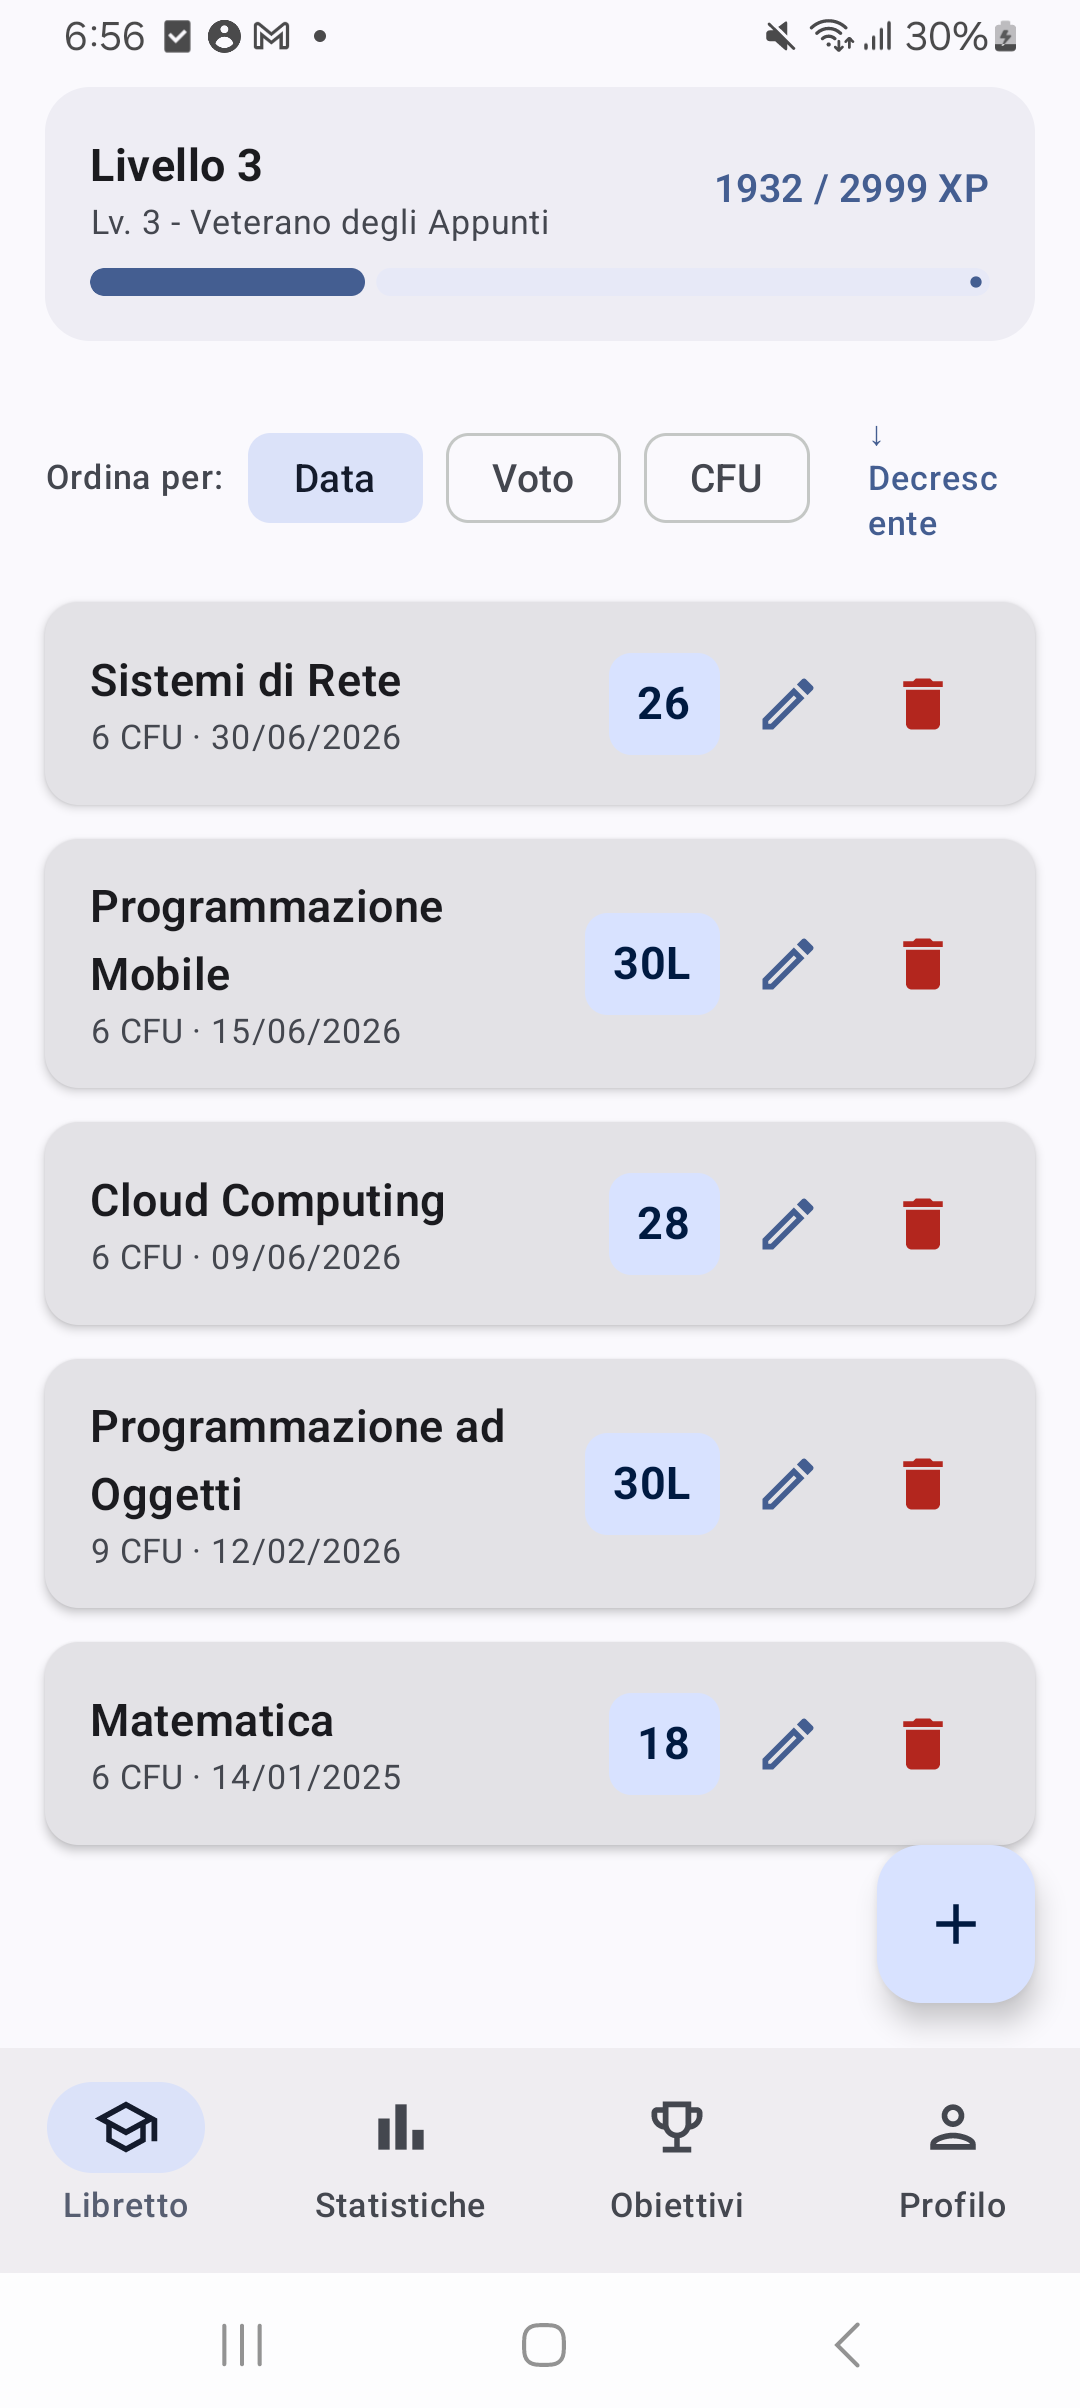
\includegraphics[width=0.42\textwidth]{libretto_screen.png}
    \hfill
    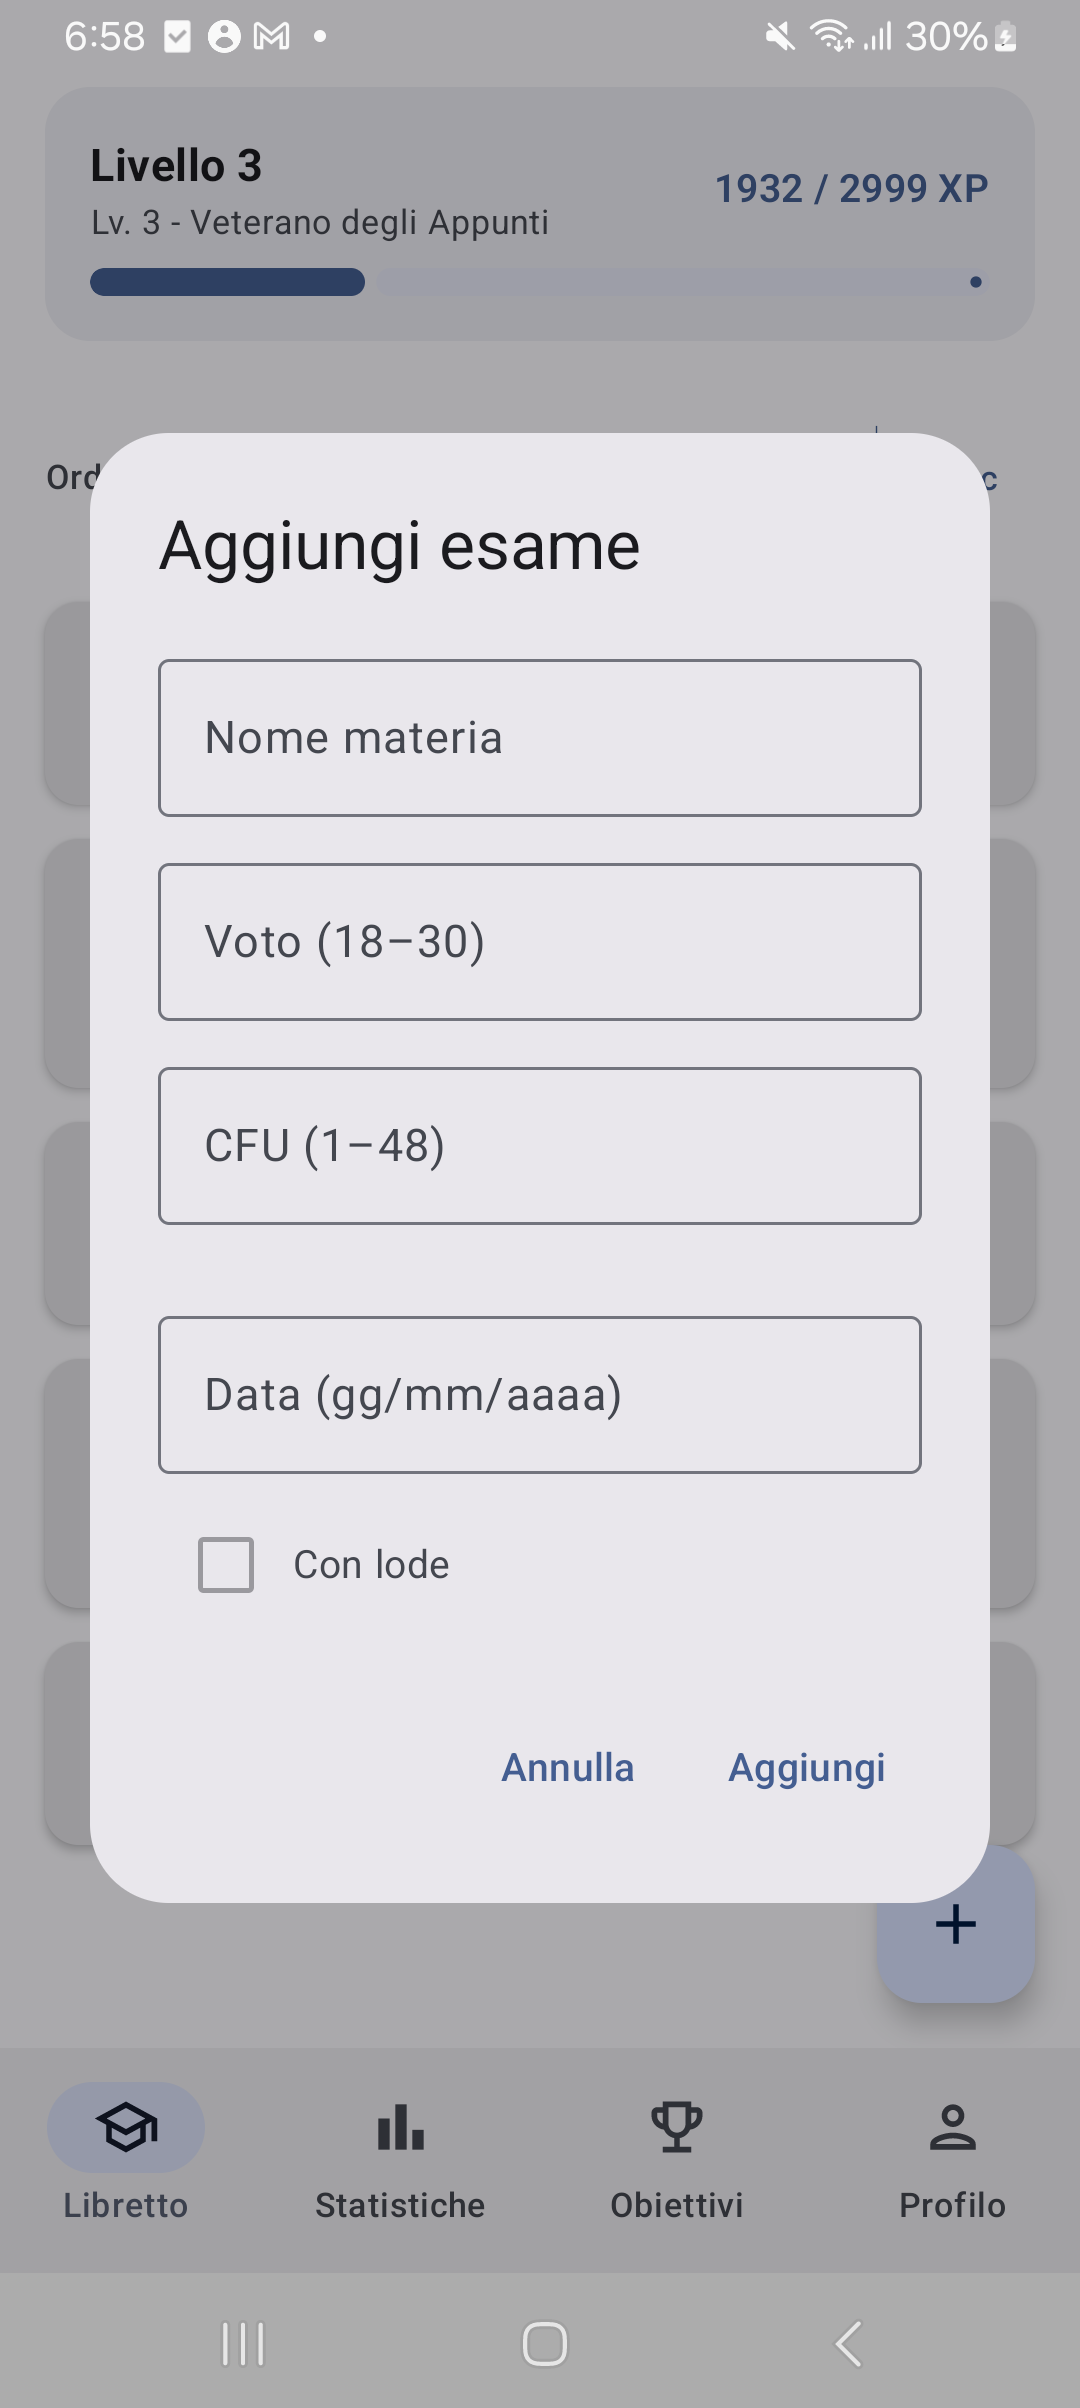
\includegraphics[width=0.42\textwidth]{libretto_add_dialog.png}
    \caption{Schermata Libretto esami (\texttt{LibrettoScreen}): lista reattiva con
             ordinamento configurabile (sinistra) e dialog di aggiunta esame
             (\texttt{AddEsameDialog}) con validazione in linea (destra).}
    \label{fig:libretto}
\end{figure}

\section{Architettura UI con Jetpack Compose e navigazione adattiva}

\paragraph{Problema}
A partire dall'introduzione di Jetpack Compose nel corso, il layer UI deve adottare
il paradigma dichiarativo. Occorre una struttura di navigazione che si adatti
automaticamente a smartphone, tablet e finestre ridimensionabili su desktop,
senza richiedere layout alternativi per ogni configurazione.

\paragraph{Soluzione}
Il modulo \texttt{:ui} è stato interamente convertito a Jetpack Compose.
\texttt{MainActivity} estende \texttt{ComponentActivity} e delega tutta la UI
a \texttt{setContent \{\}}, con \texttt{enableEdgeToEdge()} per il disegno
sotto le barre di sistema.

Per la navigazione adattiva si utilizza \texttt{NavigationSuiteScaffold} della
libreria \texttt{material3-adaptive-navigation-suite}: questo composable seleziona
automaticamente la modalità di navigazione più appropriata in base alle dimensioni
della finestra --- Bottom Navigation Bar su smartphone in verticale, Navigation Rail
su tablet e in orizzontale, Navigation Drawer su schermi grandi.
Il pattern segue esattamente quello insegnato nel corso e soddisfa il requisito
di responsiveness senza alcun codice condizionale esplicito.

\begin{lstlisting}
NavigationSuiteScaffold(
    navigationSuiteItems = {
        AppDestinations.entries.forEach { destination ->
            item(
                icon = { Icon(destination.icon, ...) },
                label = { Text(destination.label) },
                selected = destination == currentDestination,
                onClick = { currentDestination = destination }
            )
        }
    }
) {
    when (currentDestination) {
        AppDestinations.LIBRETTO     -> LibrettoScreen(viewModel = librettoViewModel)
        AppDestinations.STATISTICHE  -> StatisticheScreen(viewModel = statisticheViewModel)
        AppDestinations.OBIETTIVI    -> ObiettiviScreen(viewModel = obiettiviViewModel)
        AppDestinations.PROFILO      -> ProfiloScreen(viewModel = profiloViewModel)
    }
}
\end{lstlisting}

\begin{figure}[H]
    \centering
    \includegraphics[width=0.42\textwidth]{nav_phone.png}
    \hfill
    \includegraphics[width=0.52\textwidth]{nav_tablet.png}
    \caption{\texttt{NavigationSuiteScaffold} in azione: Bottom Navigation Bar su
             smartphone (sinistra) e Navigation Rail su tablet/finestra larga (destra).
             Nessun codice condizionale --- il composable seleziona automaticamente
             la modalità in base alle dimensioni della finestra.}
    \label{fig:nav-adaptive}
\end{figure}

Tutti i ViewModel dell'applicazione utilizzano il pattern \texttt{ViewModelProvider.Factory}
con dependency injection manuale: il composable ospitante recupera i repository dal
\texttt{RepositoryProvider} (implementato da \texttt{CustomApplication}) e li passa
alla factory. Questo approccio migliora la testabilità --- i ViewModel non dipendono
da \texttt{Application} e possono essere istanziati in unit test con dipendenze
fittizie --- e garantisce un DI omogeneo nell'intero layer UI:

\begin{lstlisting}
val profiloViewModel: ProfiloViewModel = viewModel(
    factory = ProfiloViewModel.provideFactory(
        getSettingsUseCase = GetSettingsUseCase(settingsRepository),
        updateSettingsUseCase = UpdateSettingsUseCase(settingsRepository),
        logoutUseCase = LogoutUseCase(authRepository)
    )
)
\end{lstlisting}

Ogni ViewModel sopravvive ai cambi di configurazione (rotazione schermo,
ridimensionamento finestra su desktop) grazie al meccanismo standard di Jetpack.

\section{Autenticazione e gestione della sessione utente}

\paragraph{Problema}
L'applicazione comunica con un backend REST (Node.js/Express) che autentica tramite
JWT in cookie HTTP-only. L'app deve: (1) presentare le schermate di login e registrazione
finché l'utente non è autenticato; (2) persistere la sessione tra riavvii dell'app;
(3) non bloccare il Main Thread durante le chiamate di rete; (4) tornare
automaticamente al login in caso di sessione scaduta o assente.

\paragraph{Soluzione}
Il network layer è costruito su \textbf{Retrofit\,2 + OkHttp\,4}. OkHttp è configurato
con un \texttt{PersistentCookieJar} (SharedPreferences-backed, descritto nella
Sezione~\ref{sec:cookiejar}), che persiste e reinvia automaticamente il cookie
\texttt{token} a ogni richiesta. Il cookie è HTTP-only: non è mai accessibile
in chiaro dal codice Kotlin.

La persistenza della sessione tra riavvii è affidata a \textbf{DataStore
(Preferences)}: all'avvio il \texttt{AuthViewModel} legge il flag \texttt{is\_logged\_in}
e lo espone come \texttt{StateFlow<Boolean?>} (\texttt{null} = caricamento in corso,
\texttt{false} = non autenticato, \texttt{true} = autenticato):

\begin{lstlisting}
val sessionState: StateFlow<Boolean?> = repository.isLoggedIn()
    .map { it as Boolean? }
    .stateIn(viewModelScope, SharingStarted.Eagerly, null)
\end{lstlisting}

Il composable radice \texttt{RootNavigation} osserva \texttt{sessionState} e decide
quale schermata mostrare senza alcuna navigazione imperativa:

\begin{lstlisting}
when (sessionState) {
    null  -> CircularProgressIndicator() // DataStore non ha ancora emesso
    false -> if (showRegister) RegisterScreen(...) else LoginScreen(...)
    true  -> StudentHubApp()             // NavigationSuiteScaffold con le tab
}
\end{lstlisting}

Quando il backend restituisce una risposta di successo, \texttt{AuthRepositoryImpl}
chiama \texttt{sessionDataStore.setLoggedIn(true)}: il DataStore emette il nuovo valore,
il \texttt{StateFlow} si aggiorna e la UI transita automaticamente verso l'app
senza alcuna chiamata esplicita alla navigazione.

\begin{figure}[H]
    \centering
    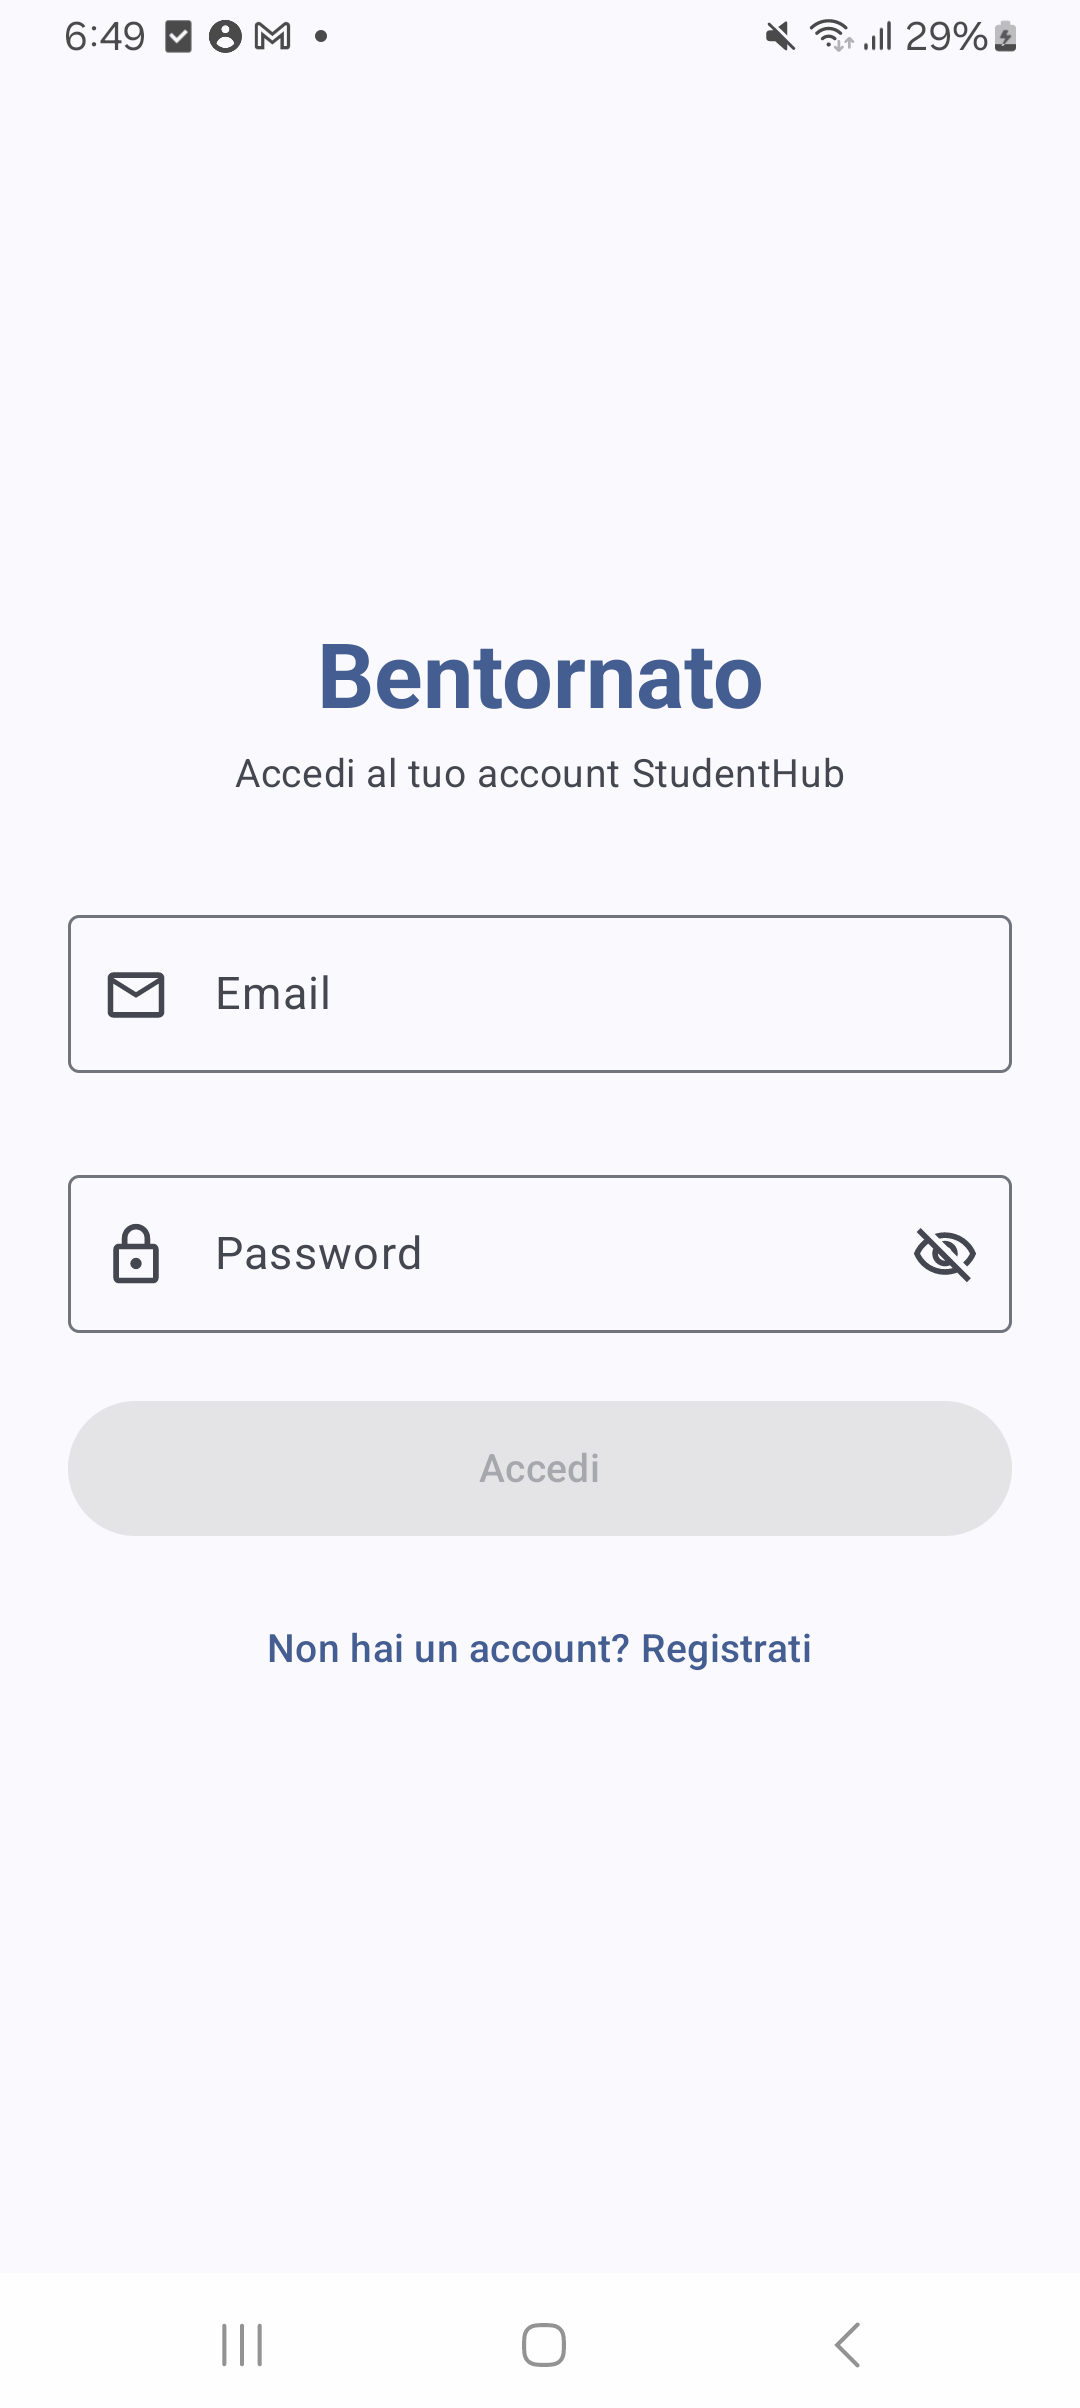
\includegraphics[width=0.40\textwidth]{login_screen.png}
    \caption{Schermata di accesso (\texttt{LoginScreen}): il pulsante e i campi si disabilitano
             durante la chiamata di rete; gli errori del server sono mostrati
             tramite \texttt{Snackbar} in italiano.}
    \label{fig:login}
\end{figure}

Il logout è implementato con lo stesso pattern dichiarativo. \texttt{LogoutUseCase}
chiama \texttt{POST /api/auth/logout} avvolto in \texttt{runCatching}: anche se
il backend non è raggiungibile, la sessione locale viene comunque invalidata
(\texttt{NetworkClient.clearCookies()} + \texttt{setLoggedIn(false)}). Il logout locale
è quindi garantito indipendentemente dalla disponibilità della rete.
\texttt{ProfiloViewModel} espone \texttt{isLoggingOut: StateFlow<Boolean>} per
disabilitare il pulsante e mostrare un indicatore di caricamento durante
l'operazione asincrona. Al termine, quando il DataStore emette \texttt{false},
\texttt{RootNavigation} torna alla schermata di login automaticamente --- nessuna
navigazione imperativa richiesta.

\section{Persistenza del cookie JWT tra riavvii}
\label{sec:cookiejar}

\paragraph{Problema}
La prima implementazione di \texttt{CookieJar} manteneva i cookie esclusivamente
in memoria. Ad ogni riavvio dell'applicazione, la cache veniva svuotata: l'utente
trovava il flag \texttt{is\_logged\_in = true} su DataStore ma le chiamate API
fallivan con 401 perché OkHttp non aveva più il cookie JWT da inviare. L'utente
risultava quindi sloggato a ogni riavvio, nonostante avesse scelto di mantenere
la sessione attiva.

\paragraph{Soluzione}
È stato sviluppato \texttt{PersistentCookieJar}, una implementazione di
\texttt{CookieJar} che serializza i cookie su \texttt{SharedPreferences} tramite
Gson e li ricarica in memoria all'inizializzazione. Le operazioni di lettura e
scrittura sono annotate \texttt{@Synchronized} per prevenire race condition sui
thread OkHttp. I cookie scaduti vengono filtrati in \texttt{loadForRequest}:

\begin{lstlisting}
@Synchronized
override fun saveFromResponse(url: HttpUrl, cookies: List<Cookie>) {
    val host = url.host
    val current = cache.getOrPut(host) { mutableListOf() }
    cookies.forEach { new ->
        current.removeAll { it.name == new.name }
        current.add(new)
    }
    prefs.edit().putString(host, serialize(current)).apply()
}

@Synchronized
override fun loadForRequest(url: HttpUrl): List<Cookie> {
    val now = System.currentTimeMillis()
    return cache[url.host]
        ?.filter { !it.persistent || it.expiresAt > now }
        ?: emptyList()
}
\end{lstlisting}

Al logout, \texttt{NetworkClient.clearCookies()} svuota sia la cache in memoria
sia le \texttt{SharedPreferences}, impedendo che una sessione precedente possa
essere riutilizzata da un utente diverso sullo stesso dispositivo.

\section{Rinnovamento automatico del token JWT}

\paragraph{Problema}
Il backend emette un access token JWT con scadenza breve (15 minuti) e
un refresh token con scadenza settimanale, entrambi in cookie HTTP-only.
Senza gestione esplicita, alla scadenza dell'access token tutte le chiamate
API cominciano a restituire 401, rendendo l'app inutilizzabile senza un
logout e login manuali.

\paragraph{Soluzione}
È stato implementato un \texttt{Authenticator} OkHttp (\texttt{TokenAuthenticator})
che intercetta automaticamente ogni risposta 401. L'authenticator esegue
una chiamata sincrona a \texttt{POST /api/auth/refresh}: il \texttt{CookieJar}
invia il refresh token già presente in memoria e riceve in risposta i cookie
aggiornati, che vengono salvati automaticamente. OkHttp ritenta quindi la
request originale --- ora autorizzata --- senza che il codice applicativo ne sia
consapevole. Se il refresh fallisce (refresh token scaduto), l'authenticator
invalida la sessione tramite \texttt{SessionDataStore.setLoggedIn(false)}:
\texttt{RootNavigation} porta l'utente alla schermata di login in modo reattivo,
senza alcuna navigazione imperativa. Una guardia blocca i loop di retry:
se la request che ha fallito con 401 è già la \texttt{/auth/refresh},
l'authenticator restituisce \texttt{null} immediatamente.

\section{Sincronizzazione offline-first con WorkManager}

\paragraph{Problema}
L'utente deve poter inserire e modificare esami anche senza connessione.
Le operazioni offline non devono andare perse quando la rete torna disponibile,
anche se l'app è stata chiusa nel frattempo.

\paragraph{Soluzione}
Ogni \texttt{EsameEntity} in Room espone il campo \texttt{pendingSync: Boolean}
(default \texttt{true}). Quando la rete è disponibile, la Request viene
inviata immediatamente (add/update/delete tramite Retrofit) e
\texttt{markSynced()} aggiorna \texttt{pending\_sync = 0} e salva il
\texttt{remote\_id} assegnato dal server.
Per il caso offline, \texttt{SyncExamsWorker} (un \texttt{CoroutineWorker})
viene schedulato con \texttt{WorkManager.enqueueUniquePeriodicWork} con constraint
\texttt{NetworkType.CONNECTED}: si esegue ogni ora ma solo quando la connessione
è disponibile, anche a app chiusa. Il worker legge dalla DAO tutti i record con
\texttt{pendingSync = true} e per ognuno chiama l'endpoint corretto: POST se
\texttt{remoteId == null} (mai sincronizzato), PUT se \texttt{remoteId != null}
(esame già esistente sul server, modificato offline). In caso di errore di rete
restituisce \texttt{Result.retry()}: WorkManager riproverà automaticamente
con backoff esponenziale.

\section{Notifiche di cambio rank con LeaderboardCheckWorker}

\paragraph{Problema}
L'utente deve poter essere notificato quando la sua posizione in classifica migliora,
senza tenere l'app aperta in foreground. La notifica richiede il permesso
\texttt{POST\_NOTIFICATIONS} (introdotto in Android~13) che deve essere richiesto
a runtime con una spiegazione contestuale. Il worker deve confrontare il rank
corrente con quello precedente senza duplicare la logica di fetch già presente
nel repository.

\paragraph{Soluzione}
\texttt{LeaderboardCheckWorker} estende \texttt{CoroutineWorker} e viene schedulato
in \texttt{CustomApplication} ogni 15 minuti con constraint \texttt{CONNECTED}
e policy \texttt{ExistingPeriodicWorkPolicy.KEEP} (nessuna schedulazione duplicata
se già attiva). Il rank precedente è letto da \texttt{RankDataStore} prima della
chiamata al server; \texttt{GamificationRepositoryImpl.getUserStats()} aggiorna
\texttt{RankDataStore} come effetto collaterale della fetch; il nuovo rank viene
quindi riletto e confrontato:

\begin{lstlisting}
override suspend fun doWork(): Result {
    return try {
        val oldRank = rankDataStore.currentRank.firstOrNull()
        repository.getUserStats()   // aggiorna RankDataStore
        val newRank = rankDataStore.currentRank.firstOrNull()
        if (oldRank != null && newRank != null && newRank < oldRank) {
            showNotification("Rank Aggiornato!",
                "Sei salito in classifica! Ora sei al posto #$newRank")
        }
        Result.success()
    } catch (e: Exception) {
        Result.retry()
    }
}
\end{lstlisting}

Il permesso \texttt{POST\_NOTIFICATIONS} viene richiesto all'avvio dell'app in
\texttt{ObiettiviScreen} tramite \texttt{rememberLauncherForActivityResult}.
Prima della richiesta viene mostrato un dialog di rationale che spiega
perché la notifica è utile; l'utente può rifiutarla definitivamente e l'app
rimane pienamente funzionale (la notifica è facoltativa).

\section{Gestione dello stato durante operazioni asincrone nella UI}

\paragraph{Problema}
Durante il salvataggio delle impostazioni nella \texttt{ProfiloScreen}, il ViewModel
transita attraverso uno stato intermedio. Una prima implementazione usava uno stato
\texttt{Saving} privo di dati e recuperava le impostazioni correnti accedendo
direttamente a \texttt{viewModel.uiState.value} all'interno del composable.
Questo approccio aggira il meccanismo reattivo di Compose: l'accesso diretto a
\texttt{.value} non registra una dipendenza di recomposition e può restituire
uno snapshot stantio se lo stato cambia tra due riesecuzioni della funzione composable.

\paragraph{Soluzione}
La sealed class \texttt{ProfiloUiState} è stata ristrutturata in modo che ogni
stato porti con sé tutti i dati necessari alla UI, eliminando qualsiasi accesso
diretto al flusso dello stato:

\begin{lstlisting}
sealed class ProfiloUiState {
    object Loading : ProfiloUiState()
    data class Success(val settings: Settings) : ProfiloUiState()
    data class Saving(val previousSettings: Settings) : ProfiloUiState()
    data class Error(val message: String, val settings: Settings? = null) : ProfiloUiState()
}
\end{lstlisting}

Quando l'utente avvia il salvataggio, il ViewModel transita a \texttt{Saving(settings)}
portando le impostazioni correnti. Il composable mostra il form disabilitato con
un \texttt{CircularProgressIndicator} nel bottone senza dover accedere ad altri
\texttt{StateFlow}. Al termine dell'operazione il ViewModel emette \texttt{Success(settings)}
(o \texttt{Error}): la UI si aggiorna per recomposition in modo interamente reattivo.

\begin{figure}[H]
    \centering
    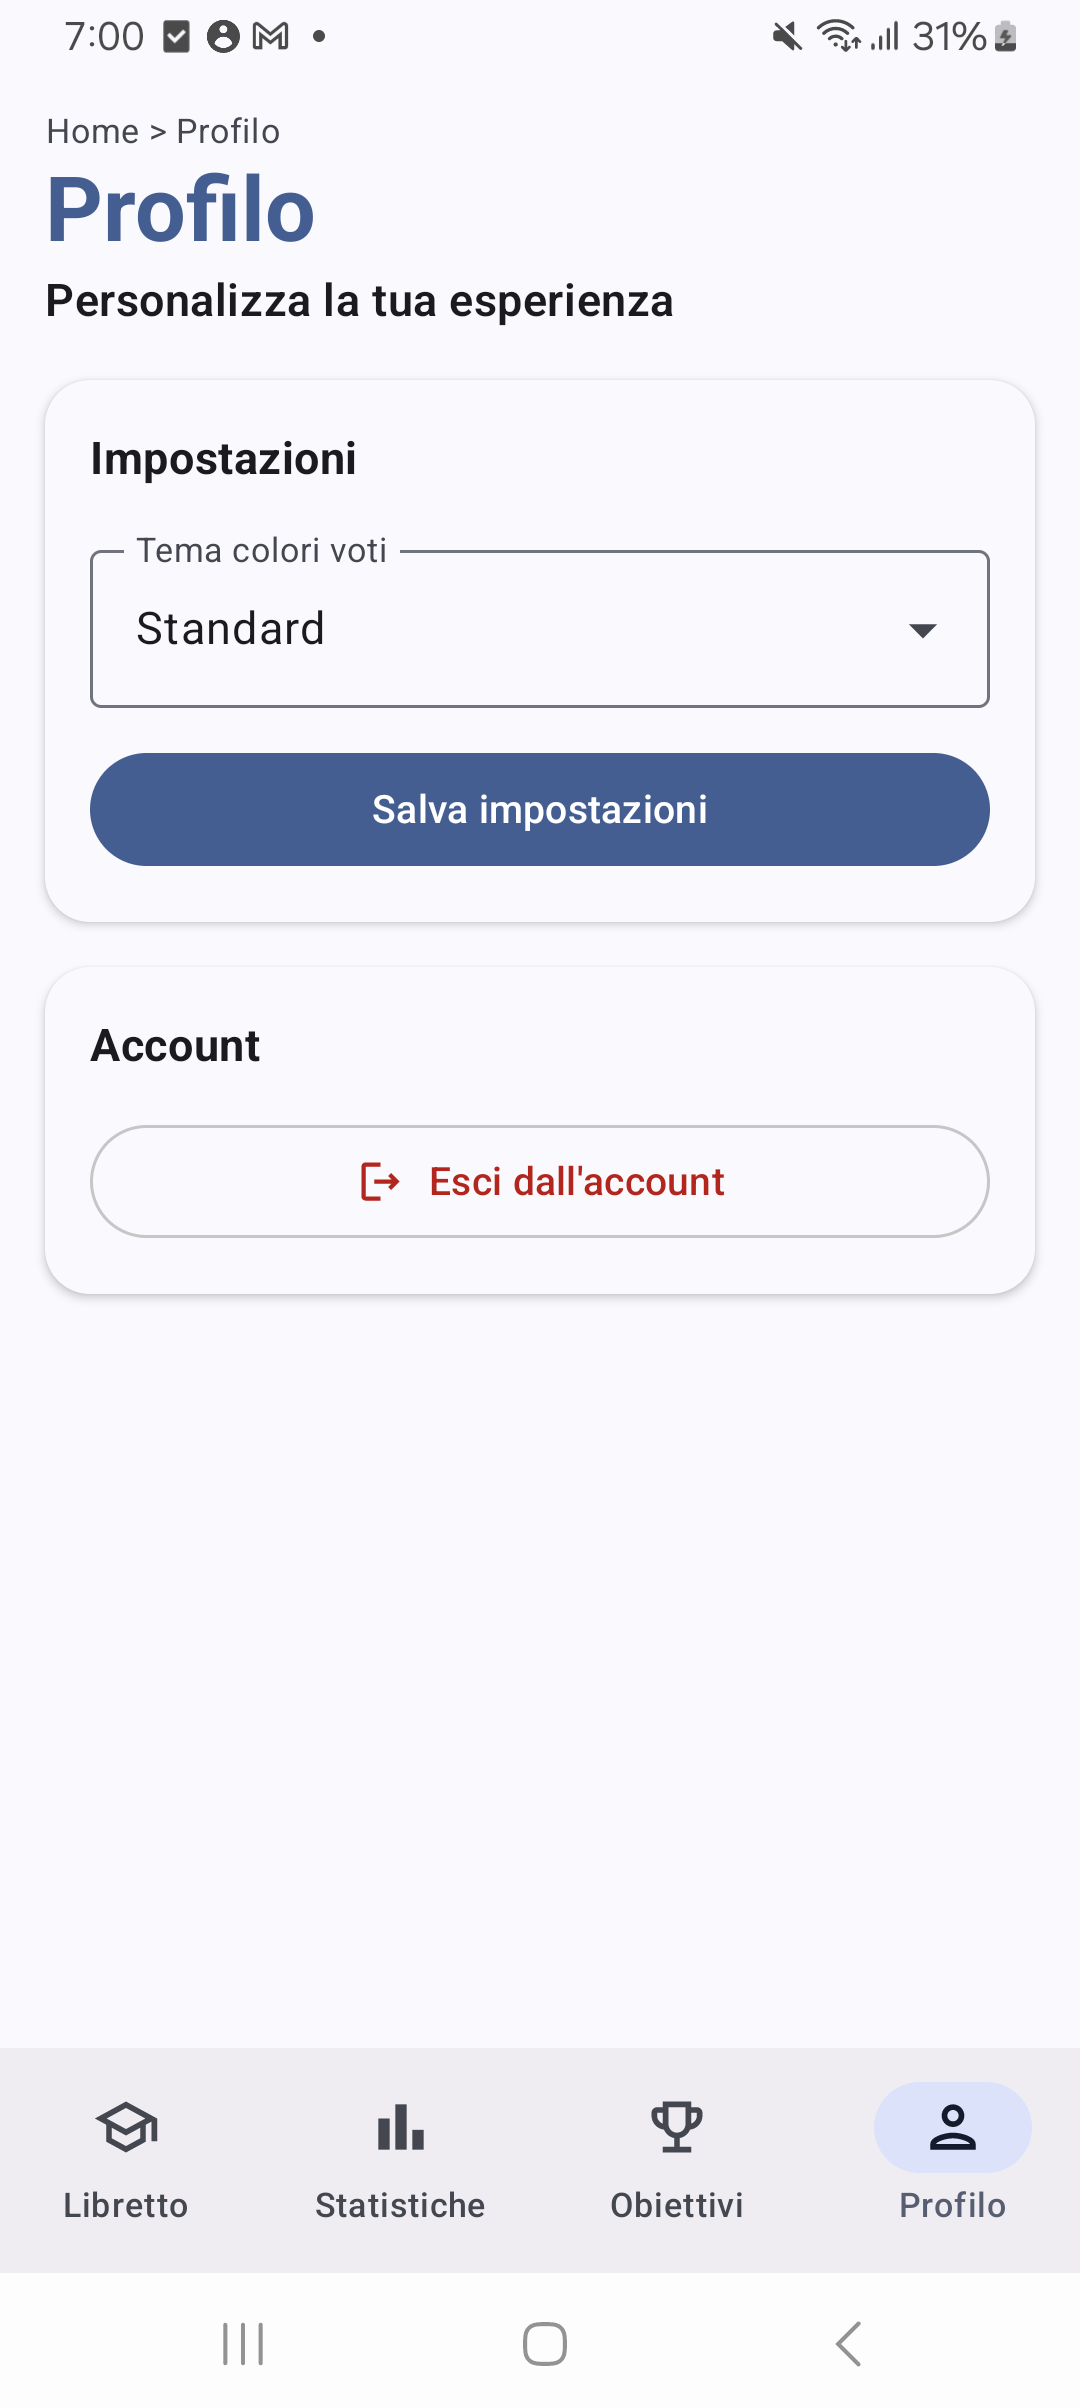
\includegraphics[width=0.42\textwidth]{profilo_screen.png}
    \caption{Schermata Profilo (\texttt{ProfiloScreen}): impostazioni tema voti,
             soglie RGB e pulsante logout. Il form viene disabilitato durante
             il salvataggio (\texttt{ProfiloUiState.Saving}) per prevenire
             modifiche concorrenti.}
    \label{fig:profilo}
\end{figure}

\section{Test unitari del layer di dominio}

\paragraph{Problema}
La correttezza dei calcoli statistici (\texttt{GetStatisticheUseCase}) non può essere
verificata solo con test manuali sull'app. È necessario garantire che le trasformazioni
sui dati producano risultati precisi (media ponderata, base di laurea, andamento
progressivo) per tutti i casi limite, e che i ViewModel gestiscano correttamente
gli stati di errore e i percorsi CRUD.

\paragraph{Soluzione}
Il modulo \texttt{:domain} non ha dipendenze Android: le classi di business logic
sono pure funzioni Kotlin testabili con JUnit\,4 e \texttt{kotlinx-coroutines-test}
senza emulatore. I ViewModel sono stati migrati da \texttt{AndroidViewModel}
a plain \texttt{ViewModel} con factory esplicita, eliminando la dipendenza da
\texttt{Application} e rendendo possibile l'istanziazione diretta nei test con
dipendenze fittizie. Sono stati scritti 29 test unitari suddivisi in cinque suite:

\begin{itemize}
    \item \textbf{GetStatisticheUseCaseTest} (6 test): verifica media ponderata, CFU totali,
    base di laurea e andamento progressivo. Usa un repository fittizio basato su
    \texttt{flowOf()}, eliminando qualsiasi dipendenza da Room.
    \item \textbf{AuthUseCaseTest} (7 test), \textbf{LibrettoViewModelTest} (7 test),
    \textbf{StatisticheViewModelTest} (4 test), \textbf{ProfiloViewModelTest} (5 test):
    copertura delle operazioni CRUD e dei percorsi di errore nei ViewModel principali,
    con repository mock forniti da Mockito-Kotlin.
\end{itemize}

\texttt{UnconfinedTestDispatcher} sostituisce \texttt{Dispatchers.Default} per
rendere i test con coroutine deterministici e privi di \texttt{delay} artificiali.

% ── CAPITOLO 4 — PUNTI FORTI E PUNTI DEBOLI ─────────────────
\chapter{Punti Forti e Punti Deboli}

\section{Punti Forti}

\begin{itemize}
    \item \textbf{Modulo \texttt{:domain} puro Kotlin}: nessuna dipendenza Android
    nel layer di business logic. I Use Cases e i calcoli statistici sono testabili
    su qualunque JVM senza emulatore, con tempi di esecuzione del test suite inferiori
    ai 5 secondi.

    \item \textbf{UI interamente reattiva}: la UI non interroga mai i dati in modo
    attivo. Ogni aggiornamento (nuovo esame, cambio XP, modifica impostazioni) viene
    propagato automaticamente da Room tramite \texttt{Flow} fino al composable,
    senza polling né notifiche manuali.

    \item \textbf{Strategia offline-first robusta}: il flag \texttt{pendingSync} e
    il campo \texttt{updated\_at} garantiscono che nessuna operazione vada persa
    anche in assenza prolungata di connessione. \texttt{SyncExamsWorker} garantisce
    l'esecuzione differita anche con l'app chiusa.

    \item \textbf{Token refresh trasparente}: \texttt{TokenAuthenticator} gestisce
    il rinnovo del JWT senza che nessun ViewModel o Use Case ne sia consapevole.
    Il codice applicativo non contiene mai logica di retry per gli errori 401.

    \item \textbf{Navigazione adattiva senza codice condizionale}: \texttt{NavigationSuiteScaffold}
    adatta automaticamente la navigazione al form factor (smartphone, tablet, desktop
    windowing) senza un singolo \texttt{if} sul tipo di schermo.

    \item \textbf{Factory pattern uniforme sui ViewModel}: tutti i ViewModel usano
    \texttt{ViewModelProvider.Factory} con DI manuale, garantendo testabilità omogenea
    e coerenza con il pattern insegnato dal corso.
\end{itemize}

\section{Punti Deboli}

\begin{itemize}
    \item \textbf{DI manuale non scalabile}: il pattern \texttt{RepositoryProvider}
    funziona per il perimetro attuale, ma con l'aggiunta di nuovi repository o
    dipendenze trasversali diventa verboso. Hilt sarebbe preferibile su un progetto
    di dimensioni maggiori.

    \item \textbf{Test di integrazione assenti}: Room DAO e \texttt{CoroutineWorker}
    non sono coperti da test automatici (richiedono rispettivamente un database
    in-memory e l'infrastruttura \texttt{WorkManagerTestInitHelper}). La copertura
    del test suite si ferma al layer domain e ViewModel.

    \item \textbf{Gestione errori di rete non granulare}: gli errori di rete
    (\texttt{IOException}), di timeout e di risposta server (4xx/5xx) vengono mappati
    sulla stessa classe \texttt{Error} nella UI. Una gerarchia di errori distinta
    permetterebbe messaggi più precisi all'utente.

    \item \textbf{\texttt{SharingStarted.Eagerly} su tutti i ViewModel}: adottato per
    risolvere un bug di StateFlow stale con Room (upstream fermato da
    \texttt{WhileSubscribed}), ma comporta che il Flow di Room rimanga sempre attivo
    anche quando la schermata non è visibile. Il trade-off è accettabile per
    il numero di ViewModel attuali.
\end{itemize}

% ── CAPITOLO 5 — MIGLIORIE E SVILUPPI FUTURI ────────────────
\chapter{Migliorie e Sviluppi Futuri}

\section{Migliorie a Breve Termine}

\begin{itemize}
    \item \textbf{Test di integrazione per Room}: aggiungere test con database
    in-memory per verificare query DAO, migration e comportamento del \texttt{Flow}
    al variare dei dati persistiti.
    \item \textbf{Gerarchia di errori di rete}: distinguere \texttt{NetworkError}
    (assenza di connessione), \texttt{TimeoutError} e \texttt{ServerError} per
    mostrare messaggi contestuali e strategie di retry differenziate nella UI.
    \item \textbf{Accessibilità}: completare i \texttt{contentDescription} su tutti
    gli elementi interattivi dei composable per il supporto agli screen reader.
    \item \textbf{Indicizzazione Room}: aggiungere \texttt{@Index} sulle colonne
    \texttt{remote\_id} e \texttt{pending\_sync} di \texttt{EsameEntity},
    utilizzate frequentemente dal \texttt{SyncExamsWorker}.
\end{itemize}

\section{Sviluppi Futuri}

\begin{itemize}
    \item \textbf{Notifiche Push via FCM}: sostituire le notifiche locali del
    \texttt{LeaderboardCheckWorker} con push server-side per notificare l'utente
    anche senza polling periodico dal dispositivo.
    \item \textbf{Widget home screen}: visualizzazione rapida di media ponderata e
    livello XP senza aprire l'app, tramite Glance API (Jetpack Compose per widget).
    \item \textbf{Importazione piano di studi}: integrazione con le API di Esse3 o
    Almaesami per pre-popolare il libretto con gli esami del piano di studi ufficiale.
    \item \textbf{Dependency Injection con Hilt}: migrazione da \texttt{RepositoryProvider}
    manuale a Hilt per migliorare la scalabilità del progetto e ridurre il boilerplate
    nelle factory dei ViewModel.
\end{itemize}

\end{document}
